%\subsection{01. Introducción}
\begin{frame}{Introducción 01/02}
\justifying
La mecánica es la ciencia física más antigua que trata tanto de los cuerpos en reposo como de aquellos en movimiento bajo la influencia de fuerzas. La rama de la mecánica que trata los cuerpos en reposo se llama estática, y la que trata de los cuerpos en movimiento se llama dinámica. La subcategoría de fluidos se define como la ciencia que estudia el comportamiento de los fluidos en reposo (estática de fluidos) o en movimiento (dinámica de fluidos).
{\tiny Tomada del libro Mecánica de Fluidos por Yunus A. Cengel, página 2.}
\end{frame}
	
\begin{frame}{Introducción 02/02}
\justifying
\begin{figure}[H]
\centering
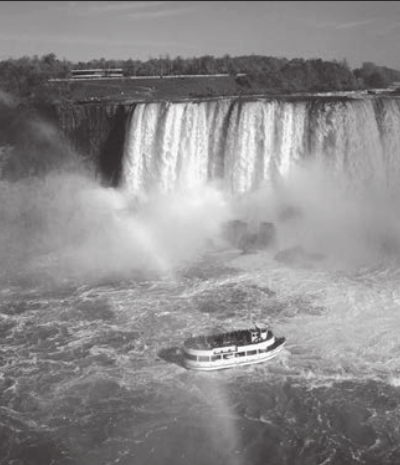
\includegraphics[scale=0.2]{Section_Files/imagenes/sec01_0101_Fig01-01.png}
\caption{La mecánica de fluidos trata de los líquidos y los gases en movimiento o en reposo.}
\label{fig: Figura1-01}
\end{figure}
{\tiny Tomada del libro Mecánica de Fluidos por Yunus A. Cengel, página 2.}
\end{frame}	

\begin{frame}{¿Qué es un fluido? 01/06}
\justifying
Una sustancia en la fase líquida o en la gaseosa se conoce como fluido. La diferencia entre un sólido y un fluido se establece con base en la capacidad de la sustancia para oponer resistencia a un esfuerzo cortante (o tangencial) aplicado que tiende a cambiar su forma.
{\tiny Tomada del libro Mecánica de Fluidos por Yunus A. Cengel, página 2.}
\end{frame}
	
\begin{frame}{¿Qué es un fluido? 02/06}
\justifying
\begin{figure}[H]
\centering
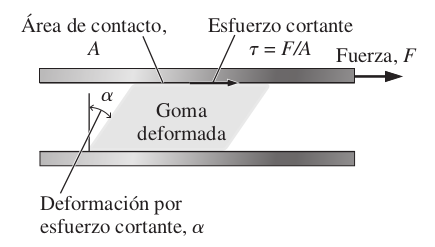
\includegraphics[scale=0.3]{Section_Files/imagenes/sec01_0101_Fig01-02.png}
\caption{Deformación de una goma para borrar colocada entre dos placas paralelas bajo la influencia de una fuerza cortante.}
\label{fig: Figura1-02}
\end{figure}
{\tiny Tomada del libro Mecánica de Fluidos por Yunus A. Cengel, página 2.}
\end{frame}
	
\begin{frame}{¿Qué es un fluido? 03/06}
\justifying
\begin{figure}[H]
\centering
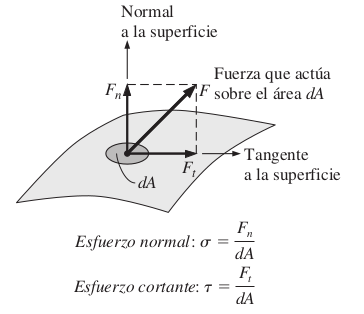
\includegraphics[scale=0.3]{Section_Files/imagenes/sec01_0101_Fig01-03.png}
\caption{Esfuerzo normal y esfuerzo cortante en la superficie de un elemento de fluido. Para los fluidos en reposo, el esfuerzo cortante es cero y la presión es el único esfuerzo normal.}
\label{fig: Figura1-03}
\end{figure}
Imagen tomada de Fundamentos y Aplicaciones de Mecánica de Fluidos de Yunus Cengel y John Cimbala.
\end{frame}	
	
\begin{frame}{¿Qué es un fluido? 04/06}
\justifying
\begin{figure}[H]
\centering
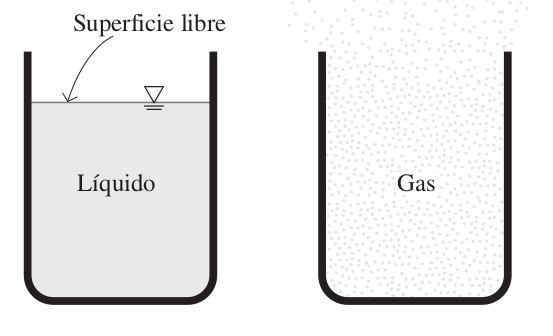
\includegraphics[scale=0.3]{Section_Files/imagenes/sec01_0101_Fig01-04.png}
\caption{A diferencia de un líquido, un gas no forma una superficie libre y se expande hasta llenar todo el espacio del que dispone.}
\label{fig: Figura1-04}
\end{figure}
Imagen tomada de Fundamentos y Aplicaciones de Mecánica de Fluidos de Yunus Cengel y John Cimbala.
\end{frame}

\begin{frame}{¿Qué es un fluido? 05/06}
\justifying
\begin{figure}[H]
\centering
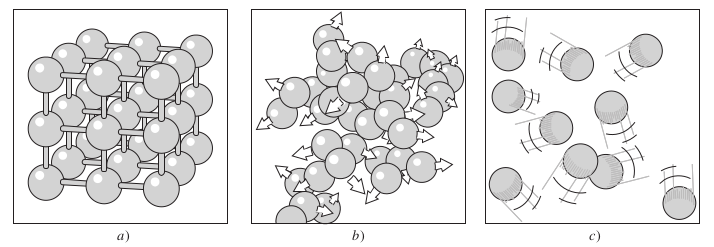
\includegraphics[scale=0.3]{Section_Files/imagenes/sec01_0101_Fig01-05.png}
\caption{ $a)$ las moléculas se encuentran en posiciones relativamente fijas en un sólido, $b)$ grupos de moléculas se mueven unos respecto a otros en la fase líquida y $c)$ las moléculas se mueven en todas las direcciones al azar en la fase gaseosa. }
\label{fig: Figura1-05}
\end{figure}
Imagen tomada de Fundamentos y Aplicaciones de Mecánica de Fluidos de Yunus Cengel y John Cimbala.
\end{frame}
	
\begin{frame}{¿Qué es un fluido? 06/06}
\justifying
\begin{figure}[H]
\centering
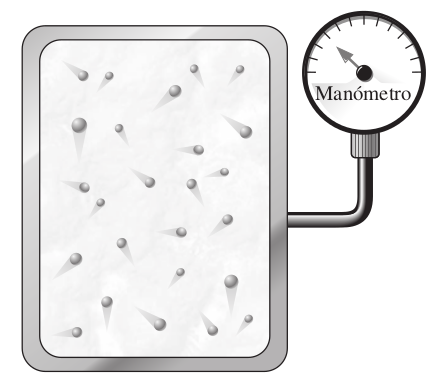
\includegraphics[scale=0.3]{Section_Files/imagenes/sec01_0101_Fig01-06.png}
\caption{En una escala microscópica, la presión se determina por la interacción de las moléculas del gas por separado. Sin embargo, se puede medir la presión a una escala macroscópica con un manómetro.}
\label{fig: Figura1-06}
\end{figure}
\end{frame}	
	
\begin{frame}{Áreas de aplicación de la mecánica de fluidos 01/03}
\justifying
La mecánica de fluidos se analiza se utiliza ampliamente en actividades cotidianas y en el diseño de sistemas modernos de ingeniería, desde aspiradoras hasta aviones supersónicos. Por lo tanto, resulta importante desarrollar una comprensión adecuada de sus principios básicos. Para empezar, la mecánica de fluidos tiene un papel vital en el cuerpo humano. El corazón bombea constantemente sangre a todas las partes del cuerpo a través de las arterias y venas, los pulmones son las regiones de flujo de aire en direcciones alternas. Los corazones artificiales, las máquinas de respiración y los sistemas de diálisis están diseñados con base en la aplicación de la mecánica de fluidos.
\end{frame}
	
\begin{frame}{Áreas de aplicación de la mecánica de fluidos 02/03}
\justifying
\begin{figure}[H]
\centering
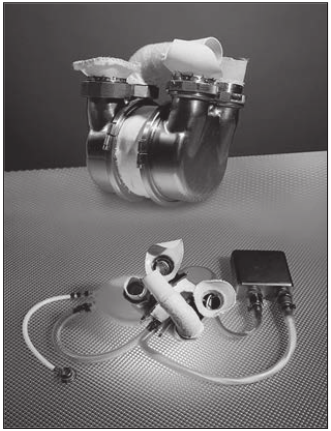
\includegraphics[scale=0.2]{Section_Files/imagenes/sec01_0101_Fig01-07.png}
\caption{La dinámica de fluidos se usa frecuentemente en el diseño de corazones artificiales. Aquí se muestra el corazón artificial de Penn State Total Electric.}
\label{fig: Figura1-07}
\end{figure}
Imagen tomada de Fundamentos y Aplicaciones de Mecánica de Fluidos de Yunus Cengel y John Cimbala.
\end{frame}
	
\begin{frame}{Áreas de aplicación de la mecánica de fluidos 03/03}
\justifying
\begin{figure}[H]
\centering
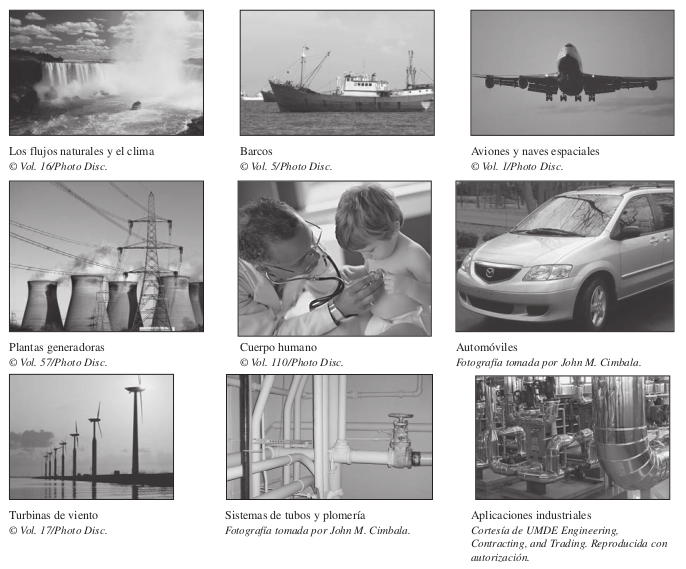
\includegraphics[scale=0.2]{Section_Files/imagenes/sec01_0101_Fig01-08.png}
\caption{Algunas áreas de aplicación de la mecánica de fluidos.}
\label{fig: Figura1-08}
\end{figure}
Imagen tomada de Fundamentos y Aplicaciones de Mecánica de Fluidos de Yunus Cengel y John Cimbala.
\end{frame}


%**********************************


%\subsection{02. Condición de no-deslizamiento}
\begin{frame}{Condición de no-deslizamiento 01/04}
\justifying
El flujo de fluidos con frecuencia se encuentra limitado por superficies sólidas y resulta importante entender de qué manera la presencia de estas superficies afecta el flujo. Se sabe que el agua de un río no puede fluir a través de rocas grandes y las rodea. Es decir, la velocidad normal del agua hacia la superfice de la roca debe ser cero y el agua que se aproxima a esa superfie en forma normal llega a detenerse por completo en ésta. Lo que no es tan obvio es que el agua que se aproxima a la roca, desde cualquier ángulo, también llega a detenerse por completo en la superfice de ella y, por consiguiente, la velocidad tangencial del agua en la superficie también es cero.
\end{frame}
	
\begin{frame}{Condición de no-deslizamiento 02/04}
\justifying
\begin{figure}[H]
\centering
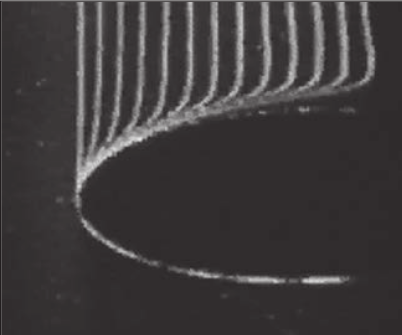
\includegraphics[scale=0.2]{Section_Files/imagenes/sec01_0101_Fig01-09.png}
\caption{Desarrollo de un perfil de velocidad debido a la condición de no-deslizamiento conforme un fluido fluye sobre el cuerpo de la parte delantera embotada.}
\label{fig: Figura1-09}
\end{figure}
Imagen tomada de Fundamentos y Aplicaciones de Mecánica de Fluidos de Yunus Cengel y John Cimbala.
\end{frame}

\begin{frame}{Condición de no-deslizamiento 03/04}
\justifying
\begin{figure}[H]
\centering
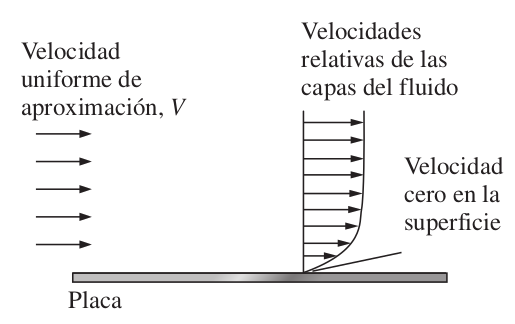
\includegraphics[scale=0.2]{Section_Files/imagenes/sec01_0101_Fig01-10.png}
\caption{Un fluido que fluye sobre una superficie en reposo llega a detenerse por completo en ésta, debido a la condición de no-deslizamiento.}
\label{fig: Figura1-10}
\end{figure}
Imagen tomada de Fundamentos y Aplicaciones de Mecánica de Fluidos de Yunus Cengel y John Cimbala.
\end{frame}
	
\begin{frame}{Condición de no-deslizamiento 04/04}
\justifying
\begin{figure}[H]
\centering
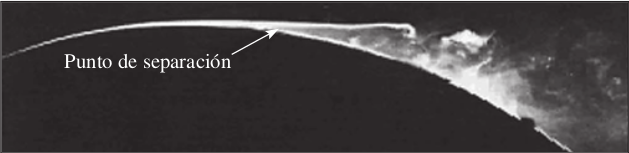
\includegraphics[scale=0.2]{Section_Files/imagenes/sec01_0101_Fig01-11.png}
\caption{Separación del flujo sobre una superficie curva.}
\label{fig: Figura1-11}
\end{figure}
Imagen tomada de Fundamentos y Aplicaciones de Mecánica de Fluidos de Yunus Cengel y John Cimbala.
\end{frame}


%**********************************


%\subsection{03. Breve historia de la mecánica de fluidos}
\begin{frame}{Breve historia de la mecánica de fluidos 01/06}
\justifying
Uno de los primeros problemas de ingeniería que enfrento la humanidad a medida que se desarrollaban las ciudades era el suministro de agua para el uso doméstico y la irrigación de los cultivos. Nuestros estilos urbanos de vida solo se pueden mantener con agua abundante y se ve con claridad, con base en la arqueología, que todas las civilizaciones sobresalientes de la prehistoria invirtieron en construcción y mantenimiento de sistemas acuíderos.
\end{frame}
	
\begin{frame}{Breve historia de la mecánica de fluidos 02/06}
\justifying
\begin{figure}[H]
\centering
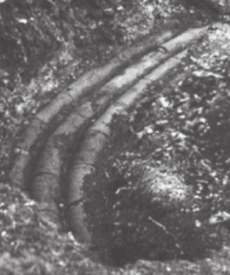
\includegraphics[scale=0.2]{Section_Files/imagenes/sec01_0101_Fig01-12.png}
\caption{Segmento de la línea de tubos de Pergamón. Cada sección de tubo de arcilla tenía de 13 a 18 cm de diámetro.}
\label{fig: Figura1-12}
\end{figure}
Imagen tomada de Fundamentos y Aplicaciones de Mecánica de Fluidos de Yunus Cengel y John Cimbala.
\end{frame}
	
\begin{frame}{Breve historia de la mecánica de fluidos 03/06}
\justifying
\begin{figure}[H]
\centering
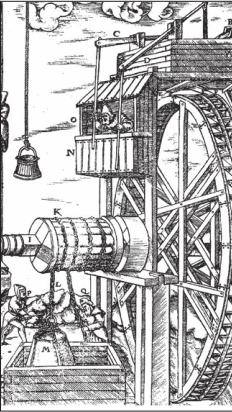
\includegraphics[scale=0.25]{Section_Files/imagenes/sec01_0101_Fig01-13.png}
\caption{Malacate de una mina impulsado por una rueda hidráulica reversible}
\label{fig: Figura1-13}
\end{figure}
\end{frame}
	
\begin{frame}{Breve historia de la mecánica de fluidos 04/06}
\justifying
\begin{figure}[H]
\centering
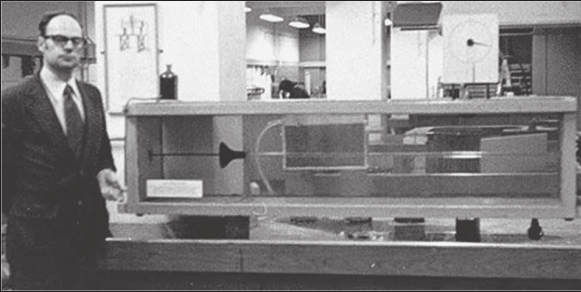
\includegraphics[scale=0.25]{Section_Files/imagenes/sec01_0101_Fig01-14.png}
\caption{Aparato original de Osbome Reynold para demostrar el inicio de la turbulencia en tubos, operado por John Lienhard, en la Universidad de Manchester, en 1975.}
\label{fig: Figura1-14}
\end{figure}
Imagen tomada de Fundamentos y Aplicaciones de Mecánica de Fluidos de Yunus Cengel y John Cimbala.
\end{frame}
	
\begin{frame}{Breve historia de la mecánica de fluidos 05/06}
\justifying
\begin{figure}[H]
\centering
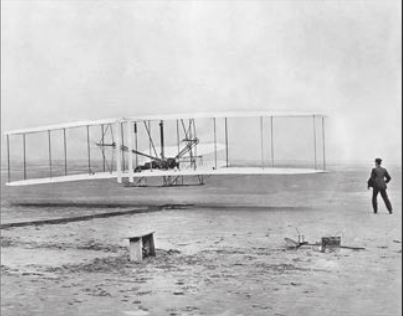
\includegraphics[scale=0.25]{Section_Files/imagenes/sec01_0101_Fig01-15.png}
\caption{Los hermanos Wright emprenden el vuelo en Kitty Hawk.}
\label{fig: Figura1-15}
\end{figure}
Imagen tomada de Fundamentos y Aplicaciones de Mecánica de Fluidos de Yunus Cengel y John Cimbala.
\end{frame}

\begin{frame}{Breve historia de la mecánica de fluidos 06/06}
\justifying
\begin{figure}[H]
\centering
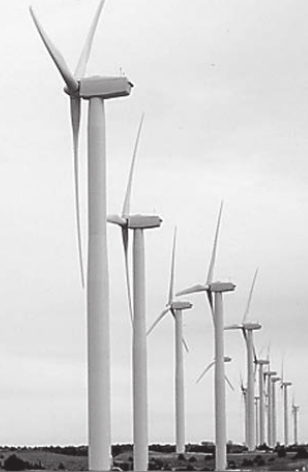
\includegraphics[scale=0.25]{Section_Files/imagenes/sec01_0101_Fig01-16.png}
\caption{El Oklahoma Wind Power Center (Centro de Energía Eólica), cerca de Woodward, consta de 68 turbinas, de 1.5 MW cada una.}
\label{fig: Figura1-16}
\end{figure}
Imagen tomada de Fundamentos y Aplicaciones de Mecánica de Fluidos de Yunus Cengel y John Cimbala.
\end{frame}


%**********************************	


%\subsection{04. Clasificación de los flujos de fluidos}
\begin{frame}{Clasificación de los flujos de fluidos}
\justifying
Al principio se definió mecánica de fluidos como la ciencia que trata del comportamiento de los fluidos en reposo o en movimiento, así como de la interacción con sólidos u otros fluidos, en las fronteras. Existe una amplia variedad de problemas del flujo de fluidos que se encuentran en la práctica y suele ser conveniente clasificarlos sobre la base de algunas características comunes, para que sea factible estudiarlos en grupos.
\end{frame}

\begin{frame}{Regiones viscosas de flujo en comparación con las no-viscosas 01/02}
\justifying
Cuando dos capas de fluido se mueven una en relación con la otra, se desarrolla una fuerza de fricción entre ellas y la capa más lenta trata de desacelerar a la más rápida. Esta resistencia interna al flujo se cuantifica mediante la propiedad de $viscosidad$ del fluido, la cual es medida de la adherencia interna de éste.
\end{frame}
	
\begin{frame}{Regiones viscosas de flujo en comparación con las no-viscosas 02/02}
\justifying
\begin{figure}[H]
\centering
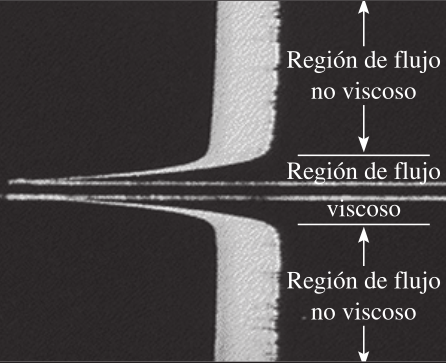
\includegraphics[scale=0.25]{Section_Files/imagenes/sec01_0101_Fig01-17.png}
\caption{Flujo de una corriente de fluido, originalmente uniforme, sobre una placa plana y las regiones de flujo viscoso (próximas a la placa en ambos lados) y de flujo no-viscoso (lejos de la placa).}
\label{fig: Figura1-17}
\end{figure}
\end{frame}
	
\begin{frame}{Flujo interno en comparación con el externo 01/02}
\justifying
Un flujo de un fluido se clasifica como interno o externo, dependiendo de si a ese fluido se le obliga a fluir en un canal confinado o sobre una superficie. El flujo de fluido no limitado sobre una superficie, como una placa, un alambre o un tubo, es flujo externo. El flujo de un tubo o ducto es flujo interno si el fluido queda por completo limitado por las superficies sólidas.
\end{frame}
	
\begin{frame}{Flujo interno en comparación con el externo 02/02}
\justifying
\begin{figure}[H]
\centering
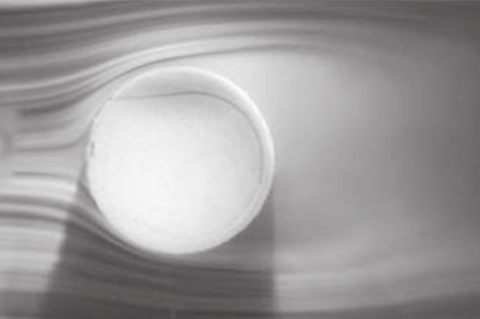
\includegraphics[scale=0.25]{Section_Files/imagenes/sec01_0101_Fig01-18.png}
\caption{Flujo externo sobre una pelota de tenis y la región de la estela turbulenta que se encuentra detrás de ella.}
\label{fig: Figura1-18}
\end{figure}
\end{frame}
	
\begin{frame}{Flujo compresible en comparación con el incompresible 01/04}
\justifying
Un flujo se clasifica como compresible o incompresible, dependiendo del nivel de variación de la densidad del flujo. La incompresibilidad es una aproximación y se dice que el flujo es incompresible si la densidad permanece aproximadamente constante a lo largo de todo el flujo. Por lo tanto el volumen de todas las porciones del fluido permanece inalterado sobre el curso de su movimiento cuando el flujo se modela como es incompresible.
\end{frame}
	
\begin{frame}{Flujo compresible en comparación con el incompresible 02/04}
\justifying
Cuando se analizan los cohetes, las naves espaciales y otros sistemas en los que intervienen flujos de gas a velocidades altas, la velocidad del flujo a menudo se expresa en términos del número adimensional Mach que se define como:
	
\begin{equation}
\ Ma = \dfrac{V}{c}
\end{equation}
\begin{itemize}
\item $V$: Velocidad del flujo.
\item $c$: Velocidad del sonido.
\end{itemize}
\end{frame}
	
\begin{frame}{Flujo compresible en comparación con el incompresible 03/04}
\justifying
En donde $c$ es la velocidad del sonido cuyo valor es de 346 m/s en el aire a temperatura ambiente al nivel del mar. Se dice que un flujo es sónico cuando $Ma = 1$, subsónico cuando Ma < 1, supersónico cuando $Ma > 1$, e hipersónico cuando $Ma >> 1$.
\end{frame}
	
	
\begin{frame}{Flujo compresible en comparación con el incompresible 04/04}
\justifying
\begin{figure}[H]
\centering
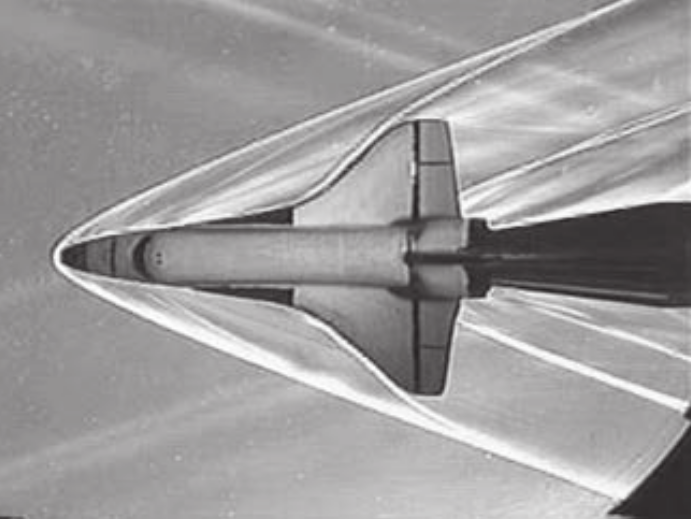
\includegraphics[scale=0.2]{Section_Files/imagenes/sec01_0101_Fig01-19.png}
\caption{Estiograma de un modelo a escala del transbordador espacial al probarse a Mach 3, en el túnel de viento supersónico del Penn State Gas Dynamics Lab. Se pueden apreciar numerosas ondas de choque oblicuas en el aire que rodea la nave.}
\label{fig: Figura1-19}
\end{figure}
\end{frame}
	
	
\begin{frame}{Flujo laminar en comparación con el turbulento 01/02}
\justifying
\begin{figure}[H]
\centering
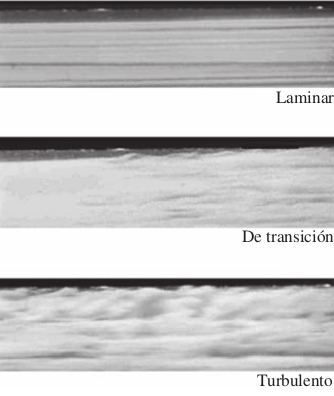
\includegraphics[scale=0.25]{Section_Files/imagenes/sec01_0101_Fig01-20.png}
\caption{Flujos laminar, de transición y turbulento.}
\label{fig: Figura1-20}
\end{figure}
Imagen tomada de Fundamentos y Aplicaciones de Mecánica de Fluidos de Yunus Cengel y John Cimbala.
\end{frame}

\begin{frame}{Flujo laminar en comparación con el turbulento 02/02}
\justifying
Algunos flujos son suaves y ordenados en tanto que otros son considerados caóticos. El movimiento intensamente ordenado de un fluido, caracterizado por capas no-alteradas de éste se conoce como laminar. La palabra laminar proviene del movimiento de partículas juntas adyacentes del fluido, en "láminas". El flujo de los fluidos intensamente viscosos, como los aceites a bajas velocidades, por lo común se presenta a velocidades altas y se caracteriza por fluctuaciones en la velocidad, se llama turbulento.
\end{frame}

\begin{frame}{Flujo natural (o no-forzado) en comparación con el forzado}
\justifying
Se dice que el flujo de un fluido es natural o forzado, dependiendo de cómo se inicia el movimiento de ese fluido. En el flujo forzado, un fluido se obliga a fluir sobre una superficie o en un tubo por medio de medios externos, como una bomba o medios naturales, como el efecto de flotación, el cual se manifiesta como la elevación del fluido más caliente y la caída del fluido más frío.
\end{frame}
	
\begin{frame}{Flujo estacionario en comparación con el no-estacionario}
\justifying
Con frecuencia, en ingeniería, se usan los términos estacionario y uniforme; en consecuencia, es importante entender con claridad sus significados. El termino estacionario implica que no hay cambio en un punto con el tiemo lo opuesto
\end{frame}
	
\begin{frame}{Flujo unidimensional, bidimensional y tridimensional (1/2)}
\justifying
\begin{figure}[H]
\centering
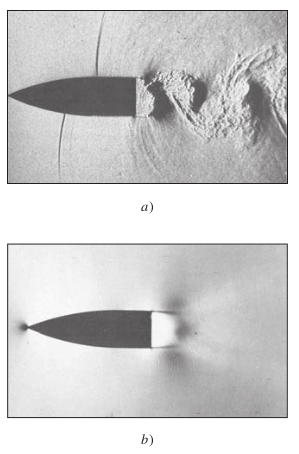
\includegraphics[scale=0.25]{Section_Files/imagenes/sec01_0101_Fig01-22.png}
\caption{Estela oscilante de un cuerpo aerodinámico de parte posterior embotada a un número de Mach de 0.6. a) Es una imagen instantánea. b) Es una imagen promediada respecto al tiempo.}
\label{fig: Figura1-22}
\end{figure}
\end{frame}
	
\begin{frame}{Flujo unidimensional, bidimensional y tridimensional (2/2)}
\justifying
\begin{figure}[H]
\centering
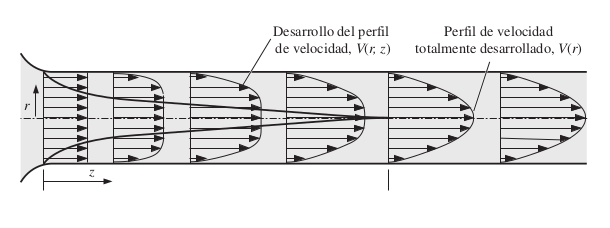
\includegraphics[scale=0.45]{Section_Files/imagenes/sec01_0101_Fig01-23.png}
\caption{Desarrollo de un perfil de velocidad en un tubo circular. $V = V(r, z)$ y, por consiguiente, el flujo es bidimensional en la región de entrada y se convierte en unidimensional corriente abajo cuando el perfil de velocidad se desarrolla totalmente y permanece inalterado en la dirección del flujo, $V = V(r)$}
\label{fig: Figura1-23}
\end{figure}
\end{frame}


%**********************************

	
%\subsection{05. Sistema de volumen de control}
\begin{frame}{Sistema de volumen de control (1/2)}
\justifying
\begin{figure}[H]
\centering
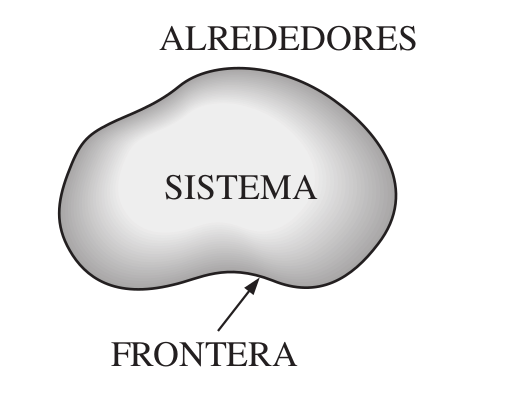
\includegraphics[scale=0.25]{Section_Files/imagenes/sec01_0101_Fig01-26.png}
\caption{Sistema, alrededores, frontera.}
\label{fig: Figura1-26}
\end{figure}
\end{frame}
	
\begin{frame}{Sistema de volumen de control (2/2)}
\justifying
\begin{figure}[H]
\centering
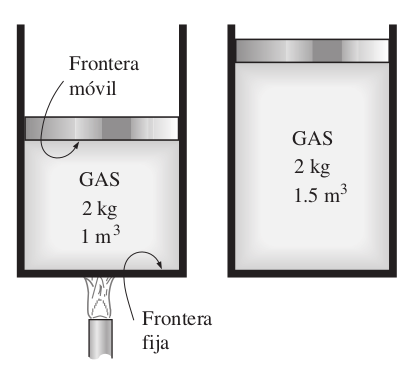
\includegraphics[scale=0.35]{Section_Files/imagenes/sec01_0101_Fig01-27.png}
\caption{Sistema cerrado con una frontera móvil.}
\label{fig: Figura1-27}
\end{figure}
\end{frame}


%**********************************	


%\subsection{06. Importancia de las dimensiones y unidades}
\begin{frame}{Algunas unidades SI}
\justifying
\begin{figure}[H]
\centering
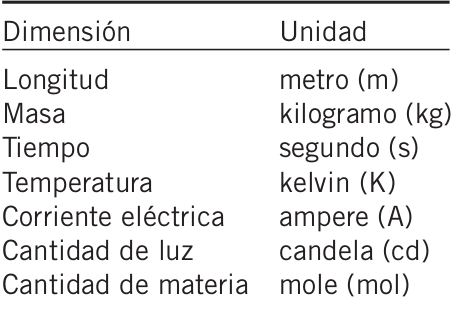
\includegraphics[scale=0.35]{Section_Files/imagenes/sec01_0101_Fig01-Tabla-1-1.png}
\caption{Las siete dimensiones fundamentales y sus unidades en el SI.}
\label{fig: Figura1-Tabla-1-1}
\end{figure}
Imagen tomada de Fundamentos y Aplicaciones de Mecánica de Fluidos de Yunus Cengel y John Cimbala.
\end{frame}
	
\begin{frame}{Homogeneidad dimensional}
\justifying
\begin{figure}[H]
\centering

\includegraphics[scale=0.25]{Section_Files/imagenes/sec01_0101_Fig01-35.png}
\caption{Para ser dimensionalmente homogéneo, todos los términos en una ecuación deben tener la misma unidad.}
\label{fig: Figura1-35}
\end{figure}
Imagen tomada de Fundamentos y Aplicaciones de Mecánica de Fluidos de Yunus Cengel y John Cimbala.
\end{frame}


%**********************************


%\subsection{07. Paquetes de software para ingeniería - CFD}
\begin{frame}{Basic elements of a CFD package}
\justifying
Son tres paquetes de elementos básicos para el CFD.
\begin{itemize}
\item Pre-proceso
\item Solver
\item Post-proceso
\end{itemize}
\end{frame}
	
\begin{frame}{Basic elements of a CFD package}
\justifying
El ciclo típico de una simulación en CFD
\begin{itemize}
\item Pre-proceso: Se escoje el modelo matemático, las ecuaciones dew interes para flujos compresibles o incompresibles, estado, ecuación de energía, flujo turbulento o laminar, etc.
\item Solver: Se ajusta una solución y resuelve los parametros, esquemas discretizados, parametros de relajación, ecuaiones lineales y finalmente se corre el solver.
\item Post-proceso: Es donde se analisa la data obtenida, se visualiza buscando entender el comportamiento de lo ocurrido.
\end{itemize}
\end{frame}